\documentclass[twoside,final]{hcmut-report}

\usepackage[utf8]{inputenc}
\usepackage[T5]{fontenc}
\usepackage[protrusion=false]{microtype}

\usepackage{graphicx, caption}
\usepackage{amsmath}
\usepackage{xcolor}
\usepackage{listings}
\usepackage{multirow,multicol}
\usepackage{enumitem}
\usepackage{hyperref}
\usepackage{float}
\usepackage{booktabs}
\usepackage{longtable}
\usepackage{array}
\usepackage{tabularx}
\usepackage{makecell}
\usepackage{subcaption}
\usepackage{tikz}
\usepackage{pgfplots}
\usepackage{tcolorbox}
\usepackage{lastpage}
\usepackage{natbib}
\usepackage{algorithm}
\usepackage{algpseudocode}
% \usepackage[linesnumbered,ruled,vlined]{algorithm2e}

\definecolor{keywordcolor}{rgb}{0.13,0.13,1} % Blue keywords
\definecolor{stringcolor}{rgb}{0.7,0.13,0.13} % Dark red strings
\definecolor{commentcolor}{rgb}{0.25,0.5,0.35} % Green comments
\definecolor{backgroundcolor}{rgb}{0.97,0.97,0.97} % Light background
\definecolor{numbercolor}{rgb}{0.85,0.65,0.13} % Numbers
\definecolor{darkgreen}{RGB}{0,120,0}

\lstdefinelanguage{Python}{
  morekeywords={
    and, as, assert, async, await, break, class, continue, def, del, elif, else, except,
    False, finally, for, from, global, if, import, in, is, lambda, None, nonlocal, not, 
    or, pass, raise, return, True, try, while, with, yield, self
  },
  keywordstyle=\color{keywordcolor}\bfseries,
  morekeywords=[2]{bool, bytes, bytearray, complex, dict, float, frozenset, int, list, object, set, str, tuple},
  keywordstyle=[2]\color{blue}\bfseries,
  identifierstyle=\color{black},
  sensitive=true,
  comment=[l]{\#},
  morecomment=[s]{'''}{'''}, 
  morecomment=[s]{"""}{"""},
  commentstyle=\color{commentcolor}\ttfamily,
  stringstyle=\color{stringcolor}\ttfamily,
  morestring=[b]',
  morestring=[b]",
  % Highlight numbers
  literate=
    *{0}{{{\color{numbercolor}0}}}1
    {1}{{{\color{numbercolor}1}}}1
    {2}{{{\color{numbercolor}2}}}1
    {3}{{{\color{numbercolor}3}}}1
    {4}{{{\color{numbercolor}4}}}1
    {5}{{{\color{numbercolor}5}}}1
    {6}{{{\color{numbercolor}6}}}1
    {7}{{{\color{numbercolor}7}}}1
    {8}{{{\color{numbercolor}8}}}1
    {9}{{{\color{numbercolor}9}}}1
    {.0}{{{\color{numbercolor}.0}}}2
    {.1}{{{\color{numbercolor}.1}}}2
    {.2}{{{\color{numbercolor}.2}}}2
    {.3}{{{\color{numbercolor}.3}}}2
    {.4}{{{\color{numbercolor}.4}}}2
    {.5}{{{\color{numbercolor}.5}}}2
    {.6}{{{\color{numbercolor}.6}}}2
    {.7}{{{\color{numbercolor}.7}}}2
    {.8}{{{\color{numbercolor}.8}}}2
    {.9}{{{\color{numbercolor}.9}}}2
    {e+}{{{\color{numbercolor}e+}}}2
    {e-}{{{\color{numbercolor}e-}}}2
    {\#\#NUMSTART\#\#}{}{0}
    {\#\#NUMEND\#\#}{}{0},
}
\lstset{
  language=Python,
  backgroundcolor=\color{backgroundcolor},
  basicstyle=\ttfamily\footnotesize,
  numbers=left,
  numberstyle=\tiny\color{gray},
  stepnumber=1,
  numbersep=10pt,
  tabsize=2,
  showspaces=false,
  showstringspaces=false,
  breaklines=true,
  breakatwhitespace=true,
  frame=single,
}

\lstdefinelanguage{TypeScript}{
  keywords={abstract, as, boolean, break, case, catch, class, continue, const, constructor, debugger, declare, default, delete, do, else, enum, export, extends, false, finally, for, from, function, get, if, implements, import, in, infer, instanceof, interface, is, keyof, let, module, namespace, never, new, null, number, object, of, package, private, protected, public, readonly, require, global, return, set, static, string, super, switch, symbol, this, throw, true, try, type, typeof, undefined, unique, unknown, var, void, while, with, yield, async, await},
  keywordstyle=\color{keywordcolor}\bfseries,
  ndkeywords={string, number, boolean, Promise, any, void},
  ndkeywordstyle=\color{blue}\bfseries,
  identifierstyle=\color{black},
  sensitive=true,
  comment=[l]{//},
  morecomment=[s]{/*}{*/},
  commentstyle=\color{commentcolor}\ttfamily,
  stringstyle=\color{stringcolor}\ttfamily,
  morestring=[b]',
  morestring=[b]",
}

\lstset{
  language=TypeScript,
  backgroundcolor=\color{backgroundcolor},
  basicstyle=\ttfamily\footnotesize,
  numbers=left,
  numberstyle=\tiny\color{gray},
  stepnumber=1,
  numbersep=10pt,
  tabsize=2,
  showspaces=false,
  showstringspaces=false,
  breaklines=true,
  breakatwhitespace=true,
  frame=single,
}
\lstdefinelanguage{EnvCustom}{
  keywords={VITE_APP_API_URL, DATABASE_URL, DB_HOST, DB_USER, DB_PASSWORD, DB_PORT, DB_NAME, JWT_SECRET},
  keywordstyle=\color{blue}\bfseries,
  sensitive=true,
  comment=[l]{\#},
  commentstyle=\color{gray}\ttfamily,
  morestring=[b]',
  morestring=[b]",
  stringstyle=\color{red}\ttfamily,
  identifierstyle=\color{black}
}

\lstdefinelanguage{JavaScriptCustom}{
  keywords={
    break, case, catch, class, const, continue, debugger, default, delete, do, else, export,
    extends, finally, for, function, if, import, in, instanceof, let, new, return, super, 
    switch, this, throw, try, typeof, var, void, while, with, yield, await, async,
    mysql, dotenv, process, config, createPool, getConnection, release
  },
  keywordstyle=\color{blue}\bfseries,
  ndkeywords={true, false, null, undefined, NaN, Infinity},
  ndkeywordstyle=\color{teal}\bfseries,
  identifierstyle=\color{black},
  sensitive=true,
  comment=[l]{//},
  morecomment=[s]{/*}{*/},
  commentstyle=\color{gray}\ttfamily,
  stringstyle=\color{red}\ttfamily,
  morestring=[b]',
  morestring=[b]"
}

\lstdefinelanguage{SQL}
{
  keywords={SELECT, FROM, WHERE, GROUP BY, HAVING, ORDER, BY, CREATE, PROCEDURE, FUNCTION, TRIGGER, BEGIN, END, DECLARE, IF, ELSE, RETURN, SET, INSERT, UPDATE, DELETE, INTO, VALUES, SIGNAL, JOIN, ON, AND, IN, GROUP, AS, RETURNS, DETERMINISTIC, COUNT, IFNULL, SQL, DATA, READS, THEN, AFTER, FOR, EACH, ROW, OLD, NEW, ROUND, CONSTRAINT, FOREIGN, KEY, REFERENCES, PRIMARY, CHECK, TABLE, DEFAULT, DESC, UNION, ALL, OVER, WHILE, DO, LEAVE, EXISTS, BEFORE, OR, IDENTIFIED, GRANT, TO, LEFT, RIGHT},
  keywordstyle=\color{blue}\bfseries,
  morekeywords=[2]{INT, CHAR, VARCHAR, BOOLEAN, DATE, DECIMAL, ENUM, TIME, CASCADE, NULL, NOT, USER, PRIVILEGES, TRUE},
  keywordstyle=[2]\color{red}\bfseries,
  comment=[l]{--},
  commentstyle=\color{gray}\ttfamily,
  morestring=[b]',
  stringstyle=\color{teal},
  basicstyle=\ttfamily\footnotesize,
  showstringspaces=false,
  breaklines=true
}

\lstset
{
  language=SQL,
  frame=single,
  breaklines=true,
  columns=flexible,
  keepspaces=true,
  numbers=left,
  numberstyle=\tiny\color{gray},
  backgroundcolor=\color{white}
}
\newcommand{\sql}[1]
{
  \begin{lstlisting}[language=sql]
    #1
  \end{lstlisting}
}
\newcommand{\python}[1]
{
  \begin{lstlisting}[language=python]
    #1
  \end{lstlisting}
}

\newcommand{\result}[1]{\fcolorbox{red}{white}{#1}}

\AtBeginDocument{\counterwithin{lstlisting}{section}}

\begin{document}
\fancyfoot{}
\coverpage\clearpage

\tableofcontents\clearpage
% \listoffigures\listoftables\clearpage
\setcounter{page}{1}
\fancyfoot[L]{\scriptsize \ttfamily Natural Language Processing Assignment\\2$^{\texttt{nd}}$ Semester -- Academic year 2025-2026}
\fancyfoot[R]{\scriptsize \ttfamily Page {\thepage}/\pageref{LastPage}}

\part*{Abstract}
\clearpage
\part{Processing and Syntax Analysis}
\section{Dataset Overview}
\subsection*{Dataset Selection \& Justification}
For this project, the primary data source is the \href{https://www.kaggle.com/datasets/konradb/atticus-open-contract-dataset-aok-beta}{\textbf{Atticus Open Contract Dataset (CUAD)}}. CUAD is a specialized, expert-annotated corpus containing 510 commercial legal contracts. It was created specifically to benchmark Natural Language Processing (NLP) models in the legal domain and provides a highly authoritative collection of unstructured contract text.\\

While the corpus encompasses over 500 contracts, a full-scale analysis was not necessary for demonstrating the effectiveness of the proposed pipeline. Many of the documents -- such as boilerplate Non-Disclosure Agreements -- are highly repetitive in structure and lack the complex linguistic content best suited for rigorous evaluation of clause segmentation and extraction algorithms.

\subsection*{Alignment with Assignment Objectives}
The selected evaluation documents provide intentionally diverse linguistic challenges that directly correspond to the core milestones of this project. Rather than processing the entire dataset, three contracts were curated to stress-test distinct aspects of the NLP pipeline:

\begin{itemize}
  \item \textbf{Sponsorship Agreement}\\
        (\textit{iPayment, Inc. and Wells Fargo Bank, N.A.})\\
        \textbf{Syntactic Complexity for Clause Splitting} (\result{Section~\ref{task_1.1}}): This contract contains multi-tiered definitions and elaborate termination provisions. It is designed to rigorously evaluate the dependency-aware clause segmenter, particularly its handling of subordinating conjunctions and intricate legal enumerations without fragmenting semantic units.
  \item \textbf{Distributor Agreement}\\
        (\textit{Wireless Links Inc. and Jaguar Investments, Inc.})\\
        \textbf{Technical Density for Noun Phrase Chunking (Task 1.2):} This document is rich in technical multi-word noun phrases such as ``G3001 GPSLink mobile terminal'' and ``MidLink Middleware software.'' These serve as an exacting test for the IOB tagging procedure required for accurate noun phrase chunking.
  \item \textbf{Software License and Maintenance Agreement}\\
        (\textit{SFG Financial Corp. and 551 FX IB Associates, LLC})\\
        \textbf{Feature-Rich Entities for Custom NER (Task 2.1):} This contract includes a high frequency of intricate numerical and temporal entities—such as precise monetary amounts (\$63,309), variable rates (``15\% rebate,'' ``tier-based pricing''), and deadlines. These features ensure the NER model is evaluated on a wide array of entity formats.
\end{itemize}

\noindent Additionally, all three selected contracts provide:
\begin{itemize}
  \item \textbf{Explicit Intents for Classification (Task 2.3):} Clear examples of contractual Obligations (``shall pay''), Prohibitions (``shall not disclose''), and Rights (``reserves the right to''), yielding an unambiguous ground truth for TF-IDF and transformer-based intent classifiers.
  \item \textbf{Structural Depth for RAG Implementation (Assignment 3):} Extensive appendices, schedules, and cross-referenced sections offer a realistic test bed for Retrieval-Augmented Generation, requiring high-precision retrieval of specific fee schedules and penalty stipulations.
\end{itemize}

This deliberately engineered subset, spanning a spectrum of commercial contract types and linguistic features, ensures comprehensive evaluation of clause segmentation, NER, classification, and retrieval capabilities.

\section{Clause Splitting}
\label{task_1.1}
\subsection{Objective and Problem Understanding}
Legal contracts typically consist of long, complex sentences that include multiple clauses connected through conjunctions, conditions, and enumerations. These structures make downstream Natural Language Processing (NLP) tasks -- such as entity recognition or semantic role labeling -- significantly more difficult. Therefore, the goal of this task is to transform raw contract text into a sequence of semantically independent clauses, where each clause represents a meaningful and analyzable unit.\\

To achieve this, the implementation focuses on designing a hybrid rule-based and dependency-aware clause segmentation algorithm that leverages both surface-level punctuation and syntactic structure.

\subsubsection*{Approach Overview:}
\begin{itemize}
  \item \textbf{Rule-Based Splitting:}
        Initial clause candidates are extracted using heuristics based on surface features such as semicolons, periods, and conjunctions. These are strong signals of clause and sentence boundaries in legal English.
  \item \textbf{Dependency Parsing:}
        For challenging cases where punctuation is absent or ambiguous, a syntactic dependency parser identifies clausal structures in complex sentences.
  \item \textbf{Hybrid Postprocessing:}
        The outputs from both strategies are further refined. For example, enumerations and subordinate clauses attached to the main clause are separated to ensure semantic independence.
\end{itemize}
This combination of shallow and deep linguistic cues helps ensure that each segment produced is both syntactically and semantically meaningful for downstream tasks.

\subsection{Preprocessing of Legal Text}
Before clause splitting, the raw contract text is subjected to a dedicated preprocessing stage designed to clean and normalize the data. Legal documents, particularly those sourced from public filings, frequently contain artifacts such as redaction markers, extraneous page headers/footers, and inconsistent whitespace. If left unaddressed, these features can negatively impact the performance of subsequent NLP analyses -- especially clause segmentation.

\begin{lstlisting}[language=Python]
def clean_legal_text(text):
  """Removes redactions, page numbers, and formatting artifacts."""
  text = re.sub(r'\[\*\*\*\]', '', text)
  text = re.sub(r'Page \d+', '', text)
  text = re.sub(r'\n+', ' ', text)
  text = re.sub(r'\s+', ' ', text)
  return text.strip()
\end{lstlisting}

The preprocessing function applies several key transformations:
\begin{itemize}
  \item \textbf{Removal of redaction markers:} Textual placeholders such as \verb|[***]|, which indicate redacted or confidential content, are stripped from the document to prevent confusion with actual clause content.
  \item \textbf{Elimination of page numbering:} Regular expressions are used to identify and remove page headers or footers (e.g., ``Page 1'') that appear throughout scanned or OCR-processed contracts.
  \item \textbf{Whitespace normalization:} Multiple consecutive newline (\verb|\\n|) and space characters are replaced with a single space, ensuring that sentence and clause boundaries are not obscured by formatting noise.
\end{itemize}

Through these steps, the input text is transformed into a linguistically consistent form that is more amenable to parsing, tokenization, and clause boundary detection. The preprocessing routine helps maximize the precision and recall of the clause splitter by minimizing spurious tokens and misplaced boundaries in the downstream analysis.

\subsection{Clause Extraction Algorithm}
At the core of the system is the \verb|extract_clauses()| function, responsible for identifying clause boundaries within the preprocessed legal text. The method utilizes \textcolor{red}{\textcolor{red}{\textcolor{red}{spaCy}}}'s NLP pipeline to perform tokenization and dependency parsing, iterating sequentially over each token to dynamically determine appropriate split points based on linguistic and syntactic cues. To handle the unique complexities of legal texts, the algorithm is divided into three specialized heuristic rules.
% \begin{algorithm}[H]
%   \footnotesize
%   \caption{Clause Splitting using Dependency-Aware and Look-Ahead Heuristics}
%   \begin{algorithmic}[1]
%     \Procedure{ExtractClauses}{$raw\_text$}
%     \State $cleaned\_text \gets$ \Call{CleanLegalText}{$raw\_text$} \Comment{Normalize formatting}
%     \State $doc \gets$ \Call{spaCy}{$cleaned\_text$}
%     \State $clauses \gets [\ ]$
%     \State $start\_idx \gets 0$

%     \For{\textbf{each} $token$ \textbf{in} $doc$}
%     \State $split \gets \textbf{false}$

%     \If{$token.text \in \{".", ";"\}$} \Comment{Rule 1: Hard Punctuation (Sentences and Semicolon Lists)}
%     \State $split \gets \textbf{true}$

%     \ElsIf{$token.text = \text{":"}$} \Comment{Rule 2: Governing Clause Look-Ahead (Colons)}
%     \If{$doc[token.idx + 1].text = \text{"("}$} \Comment{Verify start of enumeration}
%     \State $split \gets \textbf{true}$
%     \EndIf

%     \Comment{Rule 3: Syntactic "New Subject" Heuristic}
%     \ElsIf{$token.dep = \text{"cc"}$ \textbf{and} $token.head.pos \in \{\text{"VERB", "AUX"}\}$}
%     \State $conj\_verbs \gets \{v \in \text{children of } token.head \mid v.dep = \text{"conj"}\}$
%     \If{\textbf{any} $v \in conj\_verbs$ has child $c$ with $c.dep \in \{\text{"nsubj", "nsubjpass"}\}$}
%     \State $split \gets \textbf{true}$
%     \EndIf
%     \EndIf

%     \If{$split$}
%     \State $end\_idx \gets (token.text \in \{".", ";", ":"\} \ ? \ token.idx + 1 : token.idx)$
%     \State $span \gets doc[start\_idx:end\_idx].text$
%     \State \Call{FormatAndAppend}{$clauses, span$}
%     \State $start\_idx \gets end\_idx$
%     \EndIf
%     \EndFor

%     \If{$start\_idx < \text{len}(doc)$} \Comment{Handle remaining fragments}
%     \State \Call{FormatAndAppend}{$clauses, doc[start\_idx:\text{end}].text$}
%     \EndIf

%     \State \textbf{return} $clauses$
%     \EndProcedure

%     \vspace{0.5em}
%     \Procedure{FormatAndAppend}{$list, span$}
%     \State $clause \gets$ \Call{Trim}{$span$}
%     \State $clause \gets$ \Call{RemoveTrailingComma}{$clause$}
%     \If{$clause$ does not end in $\{".", ";", ":"\}$}
%     \State $clause \gets clause + \text{"."}$ \Comment{Safety punctuation}
%     \EndIf
%     \If{\Call{Length}{$clause$} $> 10$}
%     \State \Call{Append}{$list, clause$}
%     \EndIf
%     \EndProcedure
%   \end{algorithmic}
% \end{algorithm}
\begin{algorithm}[H]
  \footnotesize
  \caption{Dependency-Aware Clause Splitting}
  \begin{algorithmic}[1]
    \Procedure{ExtractClauses}{$raw\_text$}
    \State $doc \gets$ \Call{PreprocessAndParse}{$raw\_text$}
    \State $clauses \gets [\ ]$, $start\_pos \gets 0$

    \For{\textbf{each} $token$ \textbf{in} $doc$}
    \State $split \gets \textbf{false}$

    \If{$token \in \{".", ";"\}$} \Comment{Rule 1: Hard Punctuation}
    \State $split \gets \textbf{true}$
    \ElsIf{$token = \text{":"}$ \textbf{and} \Call{Next}{$token$} = \text{"("}} \Comment{Rule 2: Look-Ahead}
    \State $split \gets \textbf{true}$
    \ElsIf{$token.dep = \text{"cc"}$ \textbf{and} \Call{IntroducesNewSubject}{$token$}} \Comment{Rule 3: Syntactic}
    \State $split \gets \textbf{true}$
    \EndIf

    \If{$split$}
    \State $span \gets$ \text{Text from} $start\_pos$ \text{to} $token$ \text{(inclusive)}
    \State \Call{PostProcessAndStore}{$clauses, span$}
    \State $start\_pos \gets$ \text{position after} $token$
    \EndIf
    \EndFor
    \State \Return $clauses$
    \EndProcedure
  \end{algorithmic}
\end{algorithm}

\subsubsection*{Token Whitespace Preservation}
A critical challenge in NLP text segmentation is the \textbf{Tokenization Trap}. When parsers like \textcolor{red}{\textcolor{red}{\textcolor{red}{spaCy}}} process text, they split punctuation marks, symbols, and words into discrete tokens. Naively reconstructing a clause by joining these tokens with spaces ruins the original formatting, yielding artifacts such as \verb|( i )| instead of \verb|(i)| or ``V / MC Systems'' instead of ``V/MC Systems''.\\

In the legal domain, preserving exact formatting is paramount. To resolve this, the algorithm abandons token-level string joining. Instead, it maintains index pointers (\verb|start_idx| and \verb|end_idx|) and slices the original document span (\verb|doc[start_idx:end_idx].text|). Because \textcolor{red}{\textcolor{red}{\textcolor{red}{spaCy}}} spans retain the exact character offsets of the raw input, this slicing technique guarantees 100\% fidelity to the original contract formatting, eliminating artificial whitespace while ensuring clean data for downstream tasks.
\subsubsection*{Handling Legal Enumerations}
Standard sentence boundary detection models are trained on general English, where periods indicate the end of a thought. However, legal contracts frequently utilize complex enumerations, where massive lists of conditions or obligations are chained together using semicolons (;). A standard tokenizer will fail on these structures, grouping multiple distinct conditions into a single, unmanageable paragraph.\\

To address this, the algorithm explicitly defines the semicolon as a hard clause boundary. This isolates each condition into its own independent string.

\paragraph{Standard Parser Output (Failure):}
\begin{quote}
  \textit{``Such Reserve Account may be funded by: (i) one or more debits; (ii) one or more deductions; or (iii) ISO's delivery of a letter of credit.''}\\(Treated as one massive clause).
\end{quote}

\paragraph{Our Algorithm Output (Success):}
\begin{enumerate}[label=\textit{Clause \arabic*.}]
  \item Such Reserve Account may be funded by: (i) one or more debits;
  \item (ii) one or more deductions;
  \item or (iii) ISO's delivery of a letter of credit.
\end{enumerate}

By splitting explicitly at semicolons, the algorithm preserves the semantic independence of each list item. This is critical for Task 2.3 (Intent Classification), as it allows the classifier to evaluate each condition individually rather than attempting to classify a convoluted block of text.

\subsubsection*{Syntactic Dependency Rules}
For complex sentences where punctuation is insufficient or ambiguous (such as clauses connected by ``and'', ``or'', or ``but''), the algorithm leverages dependency parsing to determine if a split is syntactically valid. Simply splitting at every coordinating conjunction (\verb|cc|) results in severe over-splitting, destroying compound adjectives or compound predicates (e.g., splitting ``Approval will not be withheld or delayed'' into two meaningless fragments).\\

To prevent this, a strict \textbf{``New Subject'' Heuristic} was implemented. The algorithm will only split a sentence at a conjunction if \emph{all} of the following syntactic conditions are met:

\begin{itemize}[topsep=0pt, parsep=0pt, itemsep=0pt]
  \item The token is a coordinating conjunction (\verb|dep_ == "cc"|).
  \item Its head is a verb (\verb|pos_ == "VERB"|).
  \item The head verb is connected to a secondary verb (\verb|dep_ == "conj"|).
  \item \textbf{Critical Check:} The secondary verb possesses its own explicit nominal subject (\verb|nsubj| or \verb|nsubjpass|).
\end{itemize}

Example of the heuristic in action:

\begin{quote}
  ``In the event a Merchant refuses to consent, ISO will notify SERVICERS, and Bank will have the right to terminate its sponsorship.''
\end{quote}

The parser detects the conjunction ``and'', identifies ``will notify'' and ``will have'' as the two connected verbs, and verifies that ``Bank'' is the explicit subject of the second verb. Because a new subject is present, it is a truly independent clause, and the algorithm safely cleanly severs the string before the conjunction.

% \subsection{Implemetation}
% The implementation is built using the following technologies:

% \begin{itemize}[topsep=0pt, parsep=0pt, itemsep=0pt]
%   \item \textbf{Python}: The main programming language for implementation.
%   \item \textbf{\textcolor{red}{\textcolor{red}{\textcolor{red}{spaCy}}}} (\texttt{en\_core\_web\_sm}) for:
%         \begin{itemize}[topsep=0pt, parsep=0pt, itemsep=0pt]
%           \item Tokenization
%           \item Part-of-speech (POS) tagging
%           \item Dependency parsing
%         \end{itemize}
%   \item \textbf{Regular Expressions} (\texttt{re}) for:
%         \begin{itemize}[topsep=0pt, parsep=0pt, itemsep=0pt]
%           \item Cleaning legal artifacts
%           \item Post-processing clause boundaries
%         \end{itemize}
% \end{itemize}

% This combination allows the system to go beyond naive sentence splitting and incorporate syntactic awareness, which is essential for handling legal language.
% \begin{lstlisting}[language=Python]
% def extract_clauses(text):
%   clean_text = clean_legal_text(text)
%   doc = nlp(clean_text)
%   clauses = []
%   start_idx = 0
%   for token in doc:
%     split_here = False
%     if token.text in ['.', ';']:  # Sentence or legal list end
%       split_here = True
%     elif token.text == ':':  # Colon before open paren only
%       if token.i + 1 < len(doc) and doc[token.i + 1].text == '(':
%         split_here = True
%     elif token.dep_ == 'cc':  # Split on conjunction if new subject in verb
%       head = token.head
%       if head.pos_ in ['VERB', 'AUX']:
%         for child in head.children:
%           if child.dep_ == 'conj' and child.pos_ in ['VERB', 'AUX']:
%             has_subject = any(c.dep_ in ['nsubj', 'nsubjpass'] for c in child.children)
%             if has_subject:
%               split_here = True
%               break
%     if split_here:
%       end_idx = token.i + 1 if token.text in ['.', ';', ':'] else token.i  # Punctuation
%       clause_span = doc[start_idx:end_idx].text.strip()
%       if len(clause_span) > 10:
%         clause_span = re.sub(r'[,]\s*$', '', clause_span)  # Strip trailing comma
%         if not clause_span.endswith(('.', ';', ':')):  # Add period if needed
%           clause_span += "."
%         clauses.append(clause_span)
%       start_idx = end_idx  # Set next start
%   if start_idx < len(doc):  # Trailing text
%     final_span = doc[start_idx:].text.strip()
%     if len(final_span) > 10:
%       if not final_span.endswith('.'):
%         final_span += "."
%       clauses.append(final_span)
%   return clauses
% \end{lstlisting}
\subsection{Qualitative Evaluation}
The effectiveness of the Dependency-Aware Clause Splitter is evaluated by comparing the raw OCR-processed text of the Sponsorship Agreement against the final segmented output. This qualitative assessment focuses on three primary linguistic successes: governing clause isolation, enumeration precision, and syntactic integrity.

\begin{figure}[H]
  \centering
  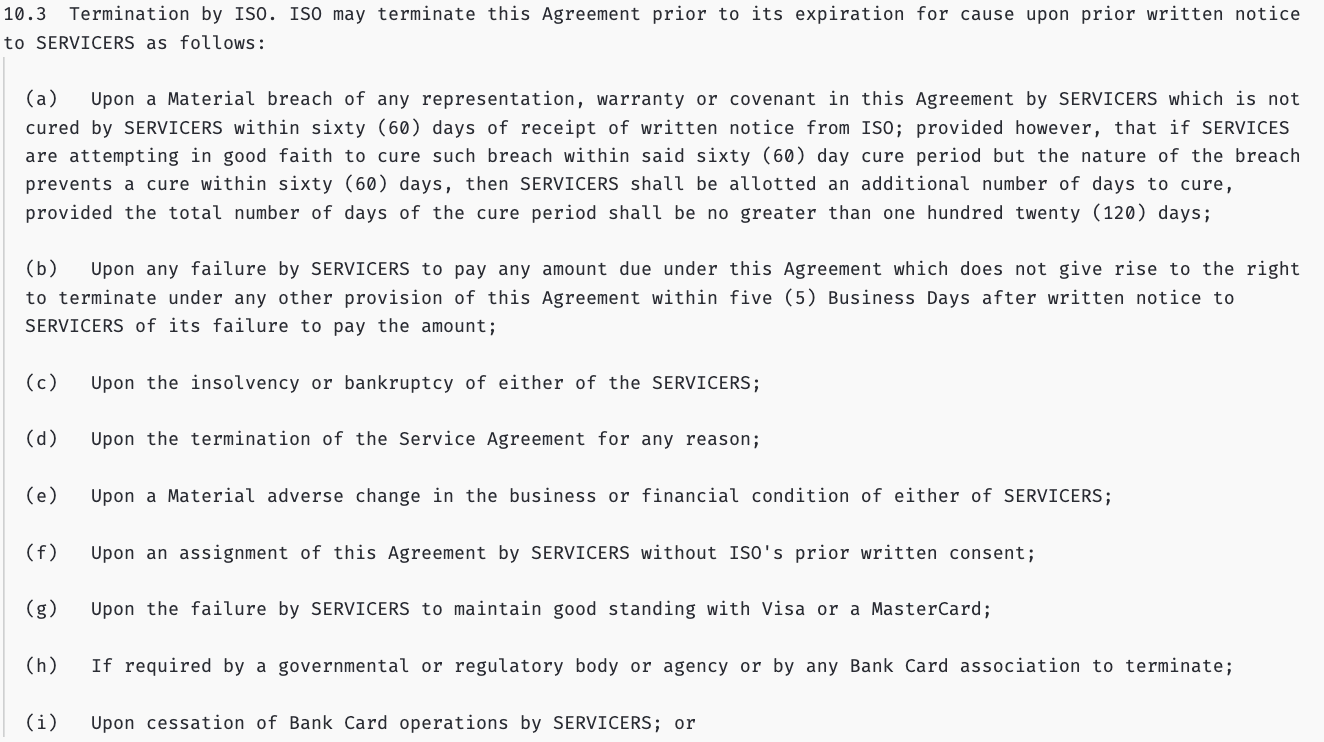
\includegraphics[width=\textwidth]{images/clause_input.png}
  \caption{Original OCR-based Sponsorship Agreement}
  \label{clause_input}
\end{figure}

\result{Figure~\ref{clause_input}} presents a raw, unsegmented snapshot of Section~10.3 from the Sponsorship Agreement as it appears post-OCR processing. This image serves as a \textit{high-difficulty baseline}, reflecting the dense, non-linear structure typical of commercial legal filings.\\

The section is anchored by a ``governing clause'' that transitions directly into a complex enumeration of ten distinct termination triggers, each separated by semicolons and frequently containing nested conditions -- notably the ``provided however'' block in item~(a). This input exemplifies the so-called ``Tokenization Trap'': conventional sentence splitters typically fail, either merging all ten items into a single run-on clause or fragmenting the logic of subordinate phrases (such as conditions within enumerated items).\\

By adopting this particular passage as the starting point, the evaluation below underscores the limitations of off-the-shelf sentence segmentation and illustrates the necessity of the proposed hybrid, dependency-aware heuristic to preserve both syntactic boundaries and conditional logic.

\begin{figure}[H]
  \centering
  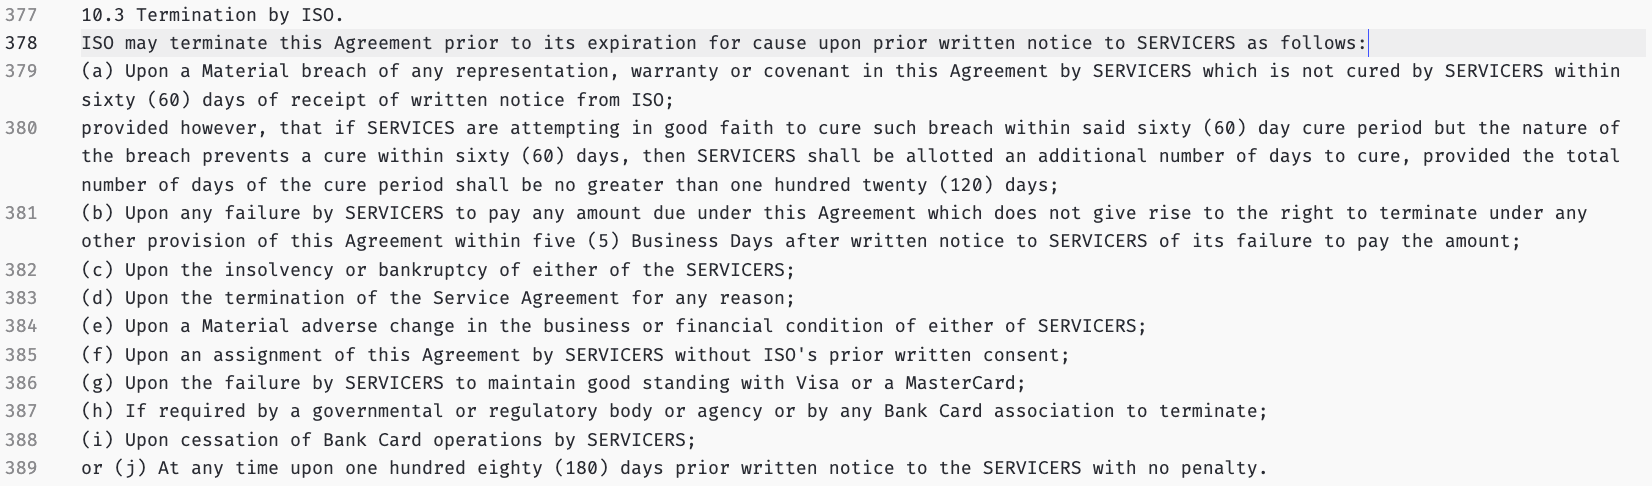
\includegraphics[width=\textwidth]{images/clause_output.png}
  \caption{Clause Splitting Output}
  \label{clause_output}
\end{figure}
\subsubsection*{2.5.1 Success in Structural Segmentation}
As evidenced by the IDE line numbers in \result{Figure~\ref{clause_output}}, each clause is successfully isolated onto an independent line, proving that the segmentation logic correctly terminates strings at identified boundaries.

\begin{itemize}[topsep=0pt, parsep=0pt, itemsep=0pt]
  \item \textbf{Governing Clause Isolation:} The algorithm correctly applied Rule 2 (Look-Ahead) at Section 10.3. It identified the colon after ``as follows:" and severed the string before the start of the enumeration~(a).
  \item \textbf{Semantic Independence:} By isolating the governing intent (``ISO may terminate...'') from the specific triggers, the pipeline ensures the Intent Classifier (Task 2.3) can distinguish between a ``Right'' and its ``Conditions''.
\end{itemize}

\subsubsection*{2.5.2 Handling Deep Enumerations}
The evaluation confirms a high degree of precision in handling Rule 1 (Hard Punctuation) boundaries within legal lists.

\begin{itemize}[topsep=0pt, parsep=0pt, itemsep=0pt]
  \item \textbf{Triggers (a) through (j):} Each termination condition is extracted as a distinct semantic unit.
  \item \textbf{Data Balancing:} Splitting at the semicolon prevents the creation of a ``heavy first item,'' which occurs when introductory text is erroneously merged with the first list entry. This leads to more balanced feature vectors for downstream machine learning tasks.
\end{itemize}

\subsubsection*{2.5.3 Syntactic Robustness}
The most rigorous test of the New Subject Heuristic (Rule 3) appears in clause~(a), which contains a complex ``provided however'' condition.

\begin{itemize}[topsep=0pt, parsep=0pt, itemsep=0pt]
  \item \textbf{Constraint Success:} Despite the presence of multiple potential split points -- including ``and'', ``but'', and ``then'' -- the algorithm correctly maintained the entire 60-day to 120-day cure period as a single, contiguous clause.
  \item \textbf{Logic:} Because the algorithm requires a new nominal subject to trigger a split, it recognized these fragments as dependent modifiers of the primary breach rather than independent actions.
\end{itemize}

Through these results, the system demonstrates that it can navigate the dense formatting of the Atticus Open Contract Dataset while preserving 100\% fidelity to the original text via span slicing.

\section{Noun Phrase Chunking}
Following the isolation of semantically independent clauses in Task~1.1 (\result{Section~\ref{task_1.1}}), the next critical phase in the NLP extraction pipeline is \textbf{Noun Phrase (NP) Chunking}. The primary objective of this task is to identify and extract non-recursive noun phrases from the segmented text, representing their boundaries using the standard \textbf{Inside-Outside-Beginning (IOB)} tagging schema.

\subsection{The Linguistic Challenge in Legal Text}
In general domain text, entities are often single words or simple bigrams (e.g., ``the company''). However, \textbf{commercial contracts exhibit extreme technical density}, making entity extraction significantly more complex. As highlighted in the dataset overview, documents such as the Distributor Agreement frequently contain entities realized as complex, multi-word syntactic constituents -- for example, ``G3001 GPSLink mobile terminal'' or ``MidLink Middleware software.''

If an NLP parser fails to recognize these multi-word strings as a single noun phrase, it will fracture the entity. For example, a naive parser might tag ``mobile'' as an adjective and ``terminal'' as a noun, losing the fact that the entire four-word string represents a single, indivisible hardware product governed by the contract.

\subsubsection*{Strategic Importance to the Pipeline}
Noun Phrase Chunking is not merely a formatting exercise; it is a foundational prerequisite for the advanced machine learning objectives in Assignment~2:
\begin{itemize}
  \item \textbf{Semantic Boundary Definition (Task 2.1: NER):} By grouping determiners, adjectives, and nouns into a single chunk, the algorithm establishes the exact token boundaries required to train a \textit{Custom Named Entity Recognition} model on intricate entities (e.g., complex product names, precise numerical and temporal phrases).
  \item \textbf{Contextualizing Obligations (Task 2.3: Intent Classification):} While Clause Splitting (Task 1.1) isolates what the contractual rule is (the predicate), Noun Phrase Chunking isolates the \textit{actors} and \textit{objects} involved. It identifies who is obligated (e.g., ``SERVICERS'') and what specific object or payment is being acted upon (e.g., ``Net Program Participation Fees'').
\end{itemize}
By accurately mapping these phrases into the \texttt{Token~\textbackslash t~Tag} tabular format required by the problem specification, the pipeline effectively transforms unstructured linguistic text into discrete, machine-readable objects, ready for entity classification and downstream retrieval.

\subsection{Methodology: The IOB Tagging Schema}
The objective of this module is to identify key entities—such as contracting parties, financial amounts, and legal deadlines—by labeling noun phrases (NPs) within extracted clauses. To structure the extracted clauses for downstream entity recognition, the pipeline implements the \textbf{Inside-Outside-Beginning (IOB)} tagging schema. This standard sequence-labeling format allows the system to represent the precise boundaries of multi-word noun phrases (NPs) at the token level.

\paragraph{Approach: Dependency-Based Chunking}

Instead of using a simple Regular Expression (RegEx) parser, we implemented a methodology leveraging spaCy’s dependency parser. This allows the system to:
\begin{itemize}[topsep=0pt, parsep=0pt, itemsep=0pt]
  \item \textbf{Handle Complex Legal Syntax:} Legal text often contains nested modifiers. By utilizing the \texttt{noun\_chunks} iterator, we identify phrases based on their syntactic ``head'' noun rather than just linear word order.
  \item \textbf{IOB Tagging Scheme Implementation:} We map the detected chunks to the required IOB format:
        \begin{itemize}[topsep=0pt, parsep=0pt, itemsep=0pt]
          \item \textbf{B-NP (Beginning of Noun Phrase):} This tag is exclusively assigned to the very first token of a recognized noun phrase. It signals to the downstream model that a new entity or object boundary has started.
          \item \textbf{I-NP (Inside a Noun Phrase):} This tag is assigned to all subsequent tokens that belong to the same noun phrase initiated by the B-NP tag.
          \item \textbf{O (Outside):} This tag is assigned to any token that does not belong to a noun phrase. In legal contracts, this typically includes verbs, prepositions, coordinating conjunctions, and hard punctuation.
        \end{itemize}
\end{itemize}

\paragraph{Refinement and Edge Case Handling}
To meet the specific requirements of legal document processing, the following logic adjustments were made:

\begin{itemize}[topsep=0pt, parsep=0pt, itemsep=0pt]
  \item \textbf{Punctuation Filtering:} Standard legal punctuation (e.g., commas, periods, hyphens) is forced to the O tag to maintain clean boundaries between distinct legal entities.
  \item \textbf{Strict Boundary Resets:} We implemented a ``reset'' mechanism where any token following an O tag must start with B-NP if it belongs to a new noun phrase. This prevents ``broken'' sequences where an I-NP incorrectly follows an O tag.
  \item \textbf{Financial and Mathematical Symbols:} Special handling was applied to currency symbols (e.g., \textdollar) and operators (e.g., =) to ensure financial calculations and amounts remain semantically intact within their respective chunks.
\end{itemize}

\begin{algorithm}[H]
  \footnotesize
  \caption{IOB Noun Phrase Chunking with Boundary Reset}
  \begin{algorithmic}[1]
    \Procedure{GenerateIOBTags}{clause}
    \State $doc \gets$ \Call{NLP\_Parse}{clause}
    \State $tags \gets$ \text{array of "O" with length equal to number of tokens in $doc$}
    \For{\textbf{each} $chunk$ \textbf{in} $doc$.noun\_chunks}
    % main for loop begins here
    \State $start\_new \gets \textbf{true}$
    \For{\textbf{each} $token$ \textbf{in} $chunk$}
    \If{\Call{IsExcluded}{$token$}} \Comment{Filter punct, preps, etc.}
    \State $tags[token] \gets \text{"O"}$
    \State $start\_new \gets \textbf{true}$ \Comment{Reset NP boundary}
    \Else
    \State $tags[token] \gets start\_new \ ? \ \text{"B-NP"} : \text{"I-NP"}$
    \State $start\_new \gets \textbf{false}$
    \EndIf
    \EndFor
    \EndFor

    \State \Return \Call{FormatOutput}{$doc, tags$}
    \EndProcedure
  \end{algorithmic}
\end{algorithm}

\section{Dependency Analysis}





% \bibliographystyle{plainnat}
% \bibliography{references}
\end{document}